\documentclass[10pt,twocolumn]{article}
\usepackage[letterpaper,margin=0.72in,columnsep=0.24in]{geometry}
\usepackage[T1]{fontenc}
\usepackage{lmodern}
\usepackage{microtype}
\usepackage{amsmath,amssymb,amsthm}
\usepackage{booktabs}
\usepackage{tabularx}
\usepackage{graphicx}
\usepackage{caption}
\usepackage{float}
\usepackage{xurl}
\usepackage[numbers,sort&compress]{natbib}
\usepackage[hidelinks]{hyperref}
\usepackage{lineno}

\newtheorem{theorem}{Theorem}
\newtheorem{corollary}[theorem]{Corollary}
\newtheorem{proposition}[theorem]{Proposition}
\newcommand{\R}{\mathbb{R}}
\newcommand{\C}{\mathbb{C}}
\newcommand{\norm}[1]{\left\lVert #1\right\rVert}
\newcommand{\tr}{\operatorname{tr}}
\newcommand{\email}[1]{\href{mailto:#1}{#1}}
\newenvironment{keywords}{\par\smallskip\noindent\textbf{Keywords. }}{\par}

\title{Parameter-Blocked Lanczos Sensitivity Replay for
Low-Launch Matrix-Function Gradients}
\author{Molena Huynh\thanks{North Carolina State University.
Email: \email{molena.huynh@jmp.com}.}}
\date{}

\hypersetup{
  pdftitle={Parameter-Blocked Lanczos Sensitivity Replay for Low-Launch Matrix-Function Gradients},
  pdfauthor={Molena Huynh}
}

\begin{document}
\setlength{\emergencystretch}{2em}
\maketitle
\linenumbers

\begin{abstract}
Differentiating a finite Lanczos matrix-function objective by tangent replay
usually processes one parameter direction at a time.  That organization is
memory economical but launches the Hermitian operator twice for every
parameter and Krylov step.  We introduce parameter-blocked tridiagonal
sensitivity replay.  A block of $q$ tangent directions is propagated as an
$n\times q$ multivector while the primal Lanczos recurrence is replayed once.
For $p$ parameters and $m$ steps, the method reduces Hamiltonian launches from
$(1+2p)m$ to
\[
 m+2m\lceil p/q\rceil,
\]
while retaining $O((q+1)n+m^2)$ working storage and the same
$O(pmn)$ column-equivalent arithmetic for sparse operators.  Full blocking
($q=p$) uses $3m$ launches independent of $p$.  We prove, by a columnwise
induction on the differentiated three-term recurrence, that every block width
produces the exact derivative of the same finite Lanczos objective in exact
arithmetic.  Consequently any certified projection error bound for scalar
replay transfers without inflation.

Four checksum-pinned PARSEC Hamiltonians from the SuiteSparse Matrix
Collection provide authenticated sparse-matrix tests.  Across four matrices
and four depths, the largest Euclidean gradient difference between full
blocking and parameterwise replay is $2.50\times10^{-16}$.  At $p=3$ and
$m=32$, nine alternating CPU repetitions give median speedups of 1.10, 1.21,
1.25, and 1.06 on matrices of dimension 769, 5,041, 8,219, and 19,896.  A
parameter sweep on SiH4 shows the explicit tradeoff: at $p=8$, launches fall
from 408 to 72 and median time falls from 0.224 to 0.103 seconds, while the
peak ambient-vector ledger rises from 10.46 to 38 vector equivalents.  At
smallest tested parameter count has little work to amortize, so launch
reduction is not stated as a universal wall-time guarantee.  The contribution is an exact
launch--memory continuum for matrix-free gradients, supported by executable
operator ledgers, accuracy tests, and real sparse matrices.
\end{abstract}

\begin{keywords}
Lanczos method, matrix-function derivative, block sparse multiplication,
matrix-free calibration, operator-launch complexity, SuiteSparse
\end{keywords}

\section{Introduction}

Krylov projection reduces a large matrix-function action to a small dense
problem.  For a Hermitian matrix $A(\theta)$, a probe $u$, and an evolution
time $t$, consider
\begin{equation}
 q(\theta)=\left|u^*\exp[-\mathrm{i}tA(\theta)]u\right|^2.
 \label{eq:objective}
\end{equation}
The Lanczos approximation replaces $A$ by an $m\times m$ tridiagonal
$T_m(\theta)$.  Matrix-function and Fr\'echet-derivative analyses for such
projections are well established
\cite{higham2008functions,saad1992analysis,almohy2009frechet,casulli2025lowmemory}.  A practical
gradient still depends on the organization of the differentiated recurrence.

Scalar tangent replay retains a constant number of ambient vectors while it
reconstructs the derivative $\dot T_{m,a}$ for parameter $a$.  Repeating that
replay for $p$ parameters avoids an $n\times m$ basis but repeats identical
primal operator applications.  On accelerators, distributed systems, and
sparse CPU kernels, launch count and memory traffic can matter independently
of the formal floating-point count.  The natural alternative is to propagate
several tangents as columns of one multivector.

This paper develops that alternative as a tunable algorithm rather than as a
fixed full batch.  Block width $q=1$ recovers parameterwise replay.  Width
$q=p$ minimizes Hamiltonian launches.  Intermediate widths occupy the
launch--memory frontier.  The exactness proof does not appeal to favorable
spectra or low tangent rank; it follows from the separability of the
differentiated scalar recurrence.  The method has no additional truncation
parameter and does not form the ambient Krylov basis or the Hamiltonian.

The evidence is organized around four claims.  Figure~\ref{fig:equivalence}
compares block and scalar gradients across matrix and depth.  Figure~\ref{fig:runtime}
reports alternating wall times on every authenticated matrix.  Figure~\ref{fig:tradeoff}
shows the exact launch and storage ledgers as parameter count grows.
Figure~\ref{fig:parameter-time} tests whether those ledgers translate to
runtime.  Tables identify the matrices and give the numerical results needed
to audit each claim.

\section{Finite Lanczos objective}

Let $v_1=u/\norm{u}_2$, $v_0=0$, and $\beta_0=0$.  The Hermitian Lanczos
recurrence is
\begin{align}
 w_j &= A v_j-\beta_{j-1}v_{j-1}, \\
 \alpha_j &= v_j^*w_j, \\
 r_j &= w_j-\alpha_jv_j, \\
 \beta_j &= \norm{r_j}_2,
 \qquad v_{j+1}=r_j/\beta_j.
 \label{eq:lanczos}
\end{align}
The resulting tridiagonal contains $\alpha_j$ on its diagonal and $\beta_j$
on its first off-diagonals.  The finite objective is
\begin{equation}
 q_m(\theta)=\norm{u}_2^4
 \left|e_1^*\exp[-\mathrm{i}tT_m(\theta)]e_1\right|^2.
 \label{eq:finite-objective}
\end{equation}
If $G_m=\nabla_{T_m}q_m$ denotes the symmetric projected sensitivity, then
\begin{equation}
 \partial_a q_m=\tr\!\left(G_m^T\dot T_{m,a}\right),
 \qquad
 \dot T_{m,a}=\frac{\partial T_m}{\partial\theta_a}.
 \label{eq:contraction}
\end{equation}
The small matrix $G_m$ is obtained by a divided-difference evaluation of the
matrix exponential.  Only the construction of all $\dot T_{m,a}$ concerns the
large dimension.

\subsection{Differentiated recurrence}

Write $D_a=\partial A/\partial\theta_a$ and place a dot on a quantity
differentiated in direction $a$.  Differentiating~\eqref{eq:lanczos} gives
\begin{align}
 \dot w_{j,a}
 &=D_av_j+A\dot v_{j,a}
   -\dot\beta_{j-1,a}v_{j-1}-\beta_{j-1}\dot v_{j-1,a}, \\
 \dot\alpha_{j,a}
 &=2\operatorname{Re}(\dot v_{j,a}^*Av_j)
   +v_j^*D_av_j, \\
 \dot r_{j,a}
 &=\dot w_{j,a}-\dot\alpha_{j,a}v_j-\alpha_j\dot v_{j,a}, \\
 \dot\beta_{j,a}
 &=\operatorname{Re}(v_{j+1}^*\dot r_{j,a}), \\
 \dot v_{j+1,a}
 &=\frac{\dot r_{j,a}-\dot\beta_{j,a}v_{j+1}}{\beta_j}.
 \label{eq:tangent}
\end{align}
The diagonal and off-diagonal entries of $\dot T_{m,a}$ are
$\dot\alpha_{j,a}$ and $\dot\beta_{j,a}$.

\section{Parameter-blocked replay}

For an index set $I$ of at most $q$ parameters, collect tangent vectors into
\begin{equation}
 \dot V_j^{(I)}=
 \begin{bmatrix}
 \dot v_{j,a_1}&\cdots&\dot v_{j,a_{|I|}}
 \end{bmatrix}\in\C^{n\times |I|}.
\end{equation}
The primal vector $v_j$ is replayed once.  The call
$A\dot V_j^{(I)}$ is one block application, while the columns
$D_av_j$ are assembled into a derivative block.  All inner products in
\eqref{eq:tangent} become columnwise reductions.  After completing the block,
the algorithm contracts its tridiagonal tangents with $G_m$ and proceeds to
the next parameter block.

\begin{theorem}[Exact block equivalence]
Assume exact arithmetic, no Lanczos breakdown through step $m$, and an
operator routine satisfying
\begin{equation}
 A[x_1,\ldots,x_s]=[Ax_1,\ldots,Ax_s].
 \label{eq:block-linearity}
\end{equation}
For every block width $q\geq1$, parameter-blocked replay returns exactly the
same $\dot T_{m,a}$ and $\partial_aq_m$ as parameterwise tangent replay for
all $a=1,\ldots,p$.
\end{theorem}

\begin{proof}
Partition the parameters into disjoint ordered blocks.  Fix a block $I$.
At $j=1$, both algorithms use
\begin{equation}
 \dot v_{0,a}=\dot v_{1,a}=0,
 \qquad \dot\beta_{0,a}=0,
 \end{equation}
for each $a\in I$.  Thus corresponding scalar and block columns agree.
Assume agreement through step $j$.  By~\eqref{eq:block-linearity}, column $a$
of the block application $A\dot V_j^{(I)}$ is precisely
$A\dot v_{j,a}$.  The derivative block has column $D_av_j$.  Every remaining
operation in~\eqref{eq:tangent} is an addition, scalar multiplication, or
columnwise inner product.  Hence the block algorithm produces the same
$\dot\alpha_{j,a}$, $\dot r_{j,a}$, $\dot\beta_{j,a}$, and
$\dot v_{j+1,a}$ as scalar replay.  Induction proves equality through $m$.
The entries of $\dot T_{m,a}$ therefore agree, and~\eqref{eq:contraction}
gives identical gradient components.
\end{proof}

Figure~\ref{fig:equivalence} is a floating-point audit of this theorem.  It is
not used as its proof.

\begin{theorem}[Launch--storage frontier]
Let $s=\lceil p/q\rceil$.  Counting an application to a vector or a
multivector as one operator launch, parameter-blocked replay uses
\begin{equation}
 L_H(m,p,q)=m+2ms
 \label{eq:launches}
\end{equation}
Hamiltonian launches and $pm$ derivative-vector applications.  Its large
working storage is $O((q+1)n)$, and its small storage is $O(pm+m^2)$.  The
column-equivalent Hamiltonian work is $(p+2)m$ vector applications.
\end{theorem}

\begin{proof}
The initial Lanczos pass uses $m$ vector launches.  Each parameter block
replays $Av_j$ and $A\dot V_j^{(I)}$ at every step, contributing $2m$ launches.
There are $s$ blocks, proving~\eqref{eq:launches}.  Each parameter contributes
one $D_av_j$ application per step, hence $pm$.  At most a constant number of
primal vectors and a constant number of $n\times q$ tangent blocks coexist,
giving $O((q+1)n)$.  Storing tangent tridiagonal coefficients requires
$O(pm)$ scalars and $G_m$ requires $O(m^2)$.  A full block application contains
at most $q$ vector columns; summing columns over all blocks yields $pm$ tangent
columns, in addition to $2m$ primal columns.
\end{proof}

\begin{corollary}[Endpoints]
Parameterwise replay ($q=1$) uses $(1+2p)m$ launches and $O(n)$ large storage.
Full blocking ($q=p$) uses $3m$ launches and $O(pn)$ large storage.
\end{corollary}

\begin{proof}
Substitute $q=1$ and $q=p$ into Theorem~2.
\end{proof}

\begin{corollary}[Inherited projection certificate]
Suppose a finite Lanczos gradient $g_m$ satisfies a certified unprojected
bound
\begin{equation}
 \norm{g-g_m}_2\leq B_m.
\end{equation}
Then every parameter-blocked result $g_m^{(q)}$ satisfies
\begin{equation}
 \norm{g-g_m^{(q)}}_2\leq B_m.
\end{equation}
\end{corollary}

\begin{proof}
Theorem~1 gives $g_m^{(q)}=g_m$ in exact arithmetic, so the two left-hand
sides are equal.  No block-width term enters the projection certificate.
\end{proof}

\section{Authenticated sparse-matrix study}

The test matrices are real-symmetric electronic-structure Hamiltonians from
the PARSEC group of the SuiteSparse Matrix Collection
\cite{davis2011suitesparse,kolodziej2019suitesparse}.  Archives are downloaded
from registered URLs and accepted only after SHA-256 verification.  Local
diagonal projectors define transparent parameter directions; they are not
device measurements.  Table~\ref{tab:data} lists the source matrices.

\begin{table}[H]
\centering
\caption{Authenticated PARSEC matrices.  Dimensions and nonzero counts refer
to the decoded symmetric matrices.}
\label{tab:data}
\small
\begin{tabular}{@{}lrrl@{}}
\toprule
Matrix & $n$ & nnz & SHA-256 prefix \\
\midrule
Si2     & 769    & 17,801  & \texttt{84e9c6f4} \\
SiH4    & 5,041  & 171,903 & \texttt{803b5243} \\
benzene & 8,219  & 242,669 & \texttt{a1f78f39} \\
Si5H12  & 19,896 & 738,598 & \texttt{895c0d8c} \\
\bottomrule
\end{tabular}
\end{table}

All accuracy tests use $p=3$, $t=8$, a fixed normalized probe, and depths
$m\in\{8,16,32,48\}$.  The reference is the independently executed
parameterwise replay.  Timing uses $m=32$, nine alternating scalar--block
repetitions, and a full parameter block.  The parameter sweep uses SiH4,
$m=24$, $p\in\{1,2,3,4,6,8\}$, and five alternating repetitions.  Medians and
0.1--0.9 timing quantiles are reported; no timing value enters the exactness
contract.

\begin{figure}[H]
\centering
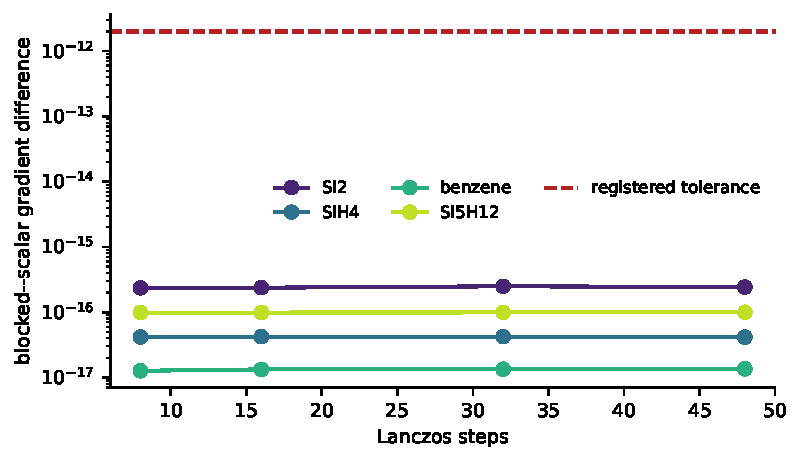
\includegraphics[width=0.92\columnwidth]{code/manuscript_assets/figures/block_equivalence.pdf}
\caption{Finite-objective equivalence across four authenticated matrices and
four depths.  The ordinate is the Euclidean difference between full-block and
parameterwise gradients.  Every value is at roundoff scale and below the
registered $2\times10^{-12}$ tolerance.}
\label{fig:equivalence}
\end{figure}

The maximum gradient difference in Figure~\ref{fig:equivalence} is
$2.50\times10^{-16}$; the maximum probability difference is zero at the
reported precision.  Every scalar run uses $7m$ Hamiltonian launches and
every full-block run uses $3m$, exactly matching Corollary~3.

\section{Runtime and parameter scaling}

Table~\ref{tab:runtime} gives the median paired timings.  Full blocking is
faster on all four matrices at $p=3$, with speedups from 1.06 to 1.25.  These
are host-specific measurements rather than asymptotic guarantees.

\begin{table}[H]
\centering
\caption{Alternating CPU timings at $p=3$ and $m=32$.}
\label{tab:runtime}
\small
\begin{tabular}{@{}lrrr@{}}
\toprule
Matrix & Scalar (s) & Block (s) & Speedup \\
\midrule
Si2     & 0.0122 & 0.0111 & 1.10 \\
SiH4    & 0.0974 & 0.0803 & 1.21 \\
benzene & 0.1404 & 0.1127 & 1.25 \\
Si5H12  & 0.2727 & 0.2575 & 1.06 \\
\bottomrule
\end{tabular}
\end{table}

\begin{figure}[H]
\centering
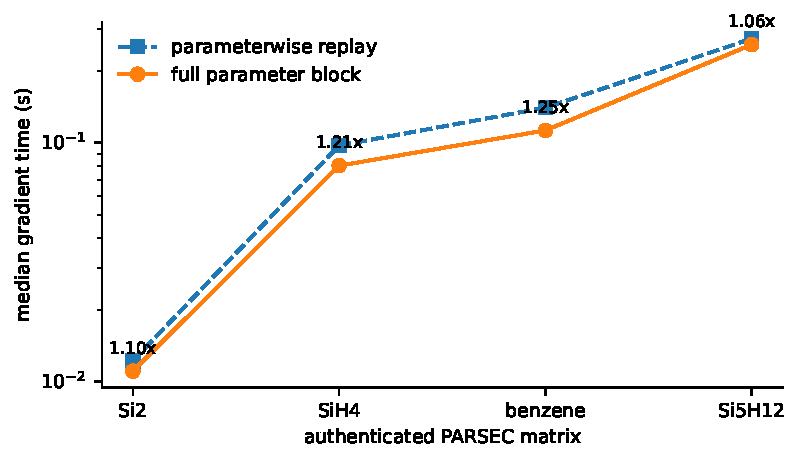
\includegraphics[width=0.92\columnwidth]{code/manuscript_assets/figures/block_runtime.pdf}
\caption{Median gradient time from nine alternating repetitions.  Labels give
the scalar-to-block ratio.  Accuracy is checked separately in
Figure~\ref{fig:equivalence}.}
\label{fig:runtime}
\end{figure}

The launch reduction has a visible but smaller wall-time effect because a
block sparse multiplication still moves and multiplies all $p$ tangent
columns.  It benefits from a shared sparse traversal and fewer interpreter and
kernel entries; it does not remove the column-equivalent arithmetic.

\begin{figure}[H]
\centering
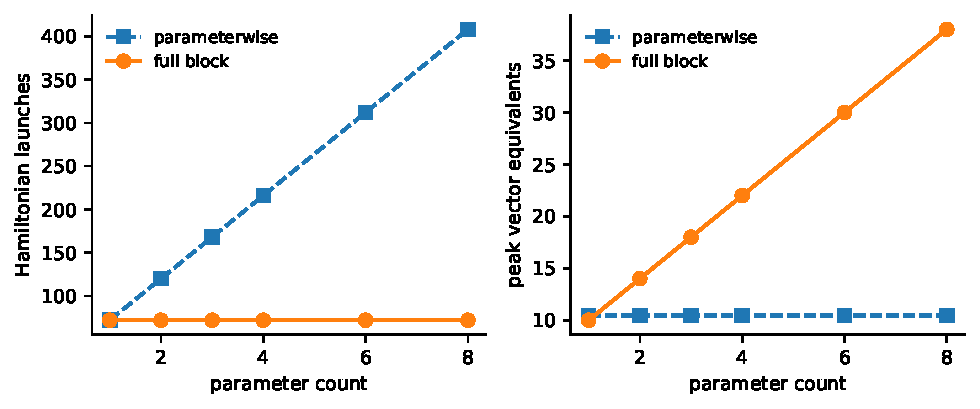
\includegraphics[width=0.86\columnwidth]{code/manuscript_assets/figures/launch_memory_tradeoff.pdf}
\caption{Exact ledger on SiH4 at $m=24$.  Full blocking holds Hamiltonian
launches at $3m=72$ as $p$ grows, compared with $(1+2p)m$ for parameterwise
replay.  The reduction is purchased with an ambient-vector ledger that grows
linearly in $p$.}
\label{fig:tradeoff}
\end{figure}

Figure~\ref{fig:tradeoff} is the computational visualization of Theorem~2.
At $p=8$, scalar replay uses 408 launches and 10.46 vector equivalents in the
released allocation model.  Full blocking uses 72 launches and 38 vector
equivalents.  Intermediate $q$ values permit a memory cap to be imposed
without changing the finite gradient.

\begin{figure}[H]
\centering
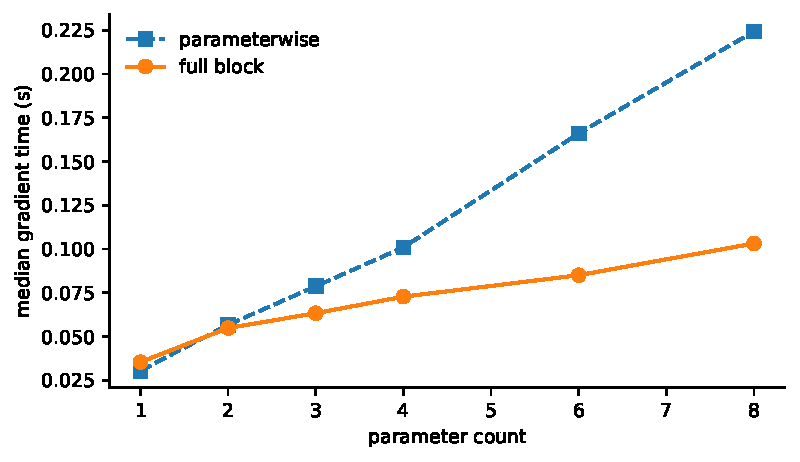
\includegraphics[width=0.86\columnwidth]{code/manuscript_assets/figures/parameter_runtime.pdf}
\caption{Measured SiH4 parameter scaling.  Full blocking gives a small timing
difference at one and two parameters and an increasing separation thereafter.
The curve is a host-specific consequence of the exact launch ledger.}
\label{fig:parameter-time}
\end{figure}

At $p=8$, median time decreases from 0.224 to 0.103 seconds.  At $p=2$, it
changes from 0.0568 to 0.0549 seconds.  Launch count is therefore a useful
mechanistic predictor, not a sufficient performance theorem.  The measured
crossover depends on sparse-kernel implementation, matrix size, and memory
hierarchy.

\section{Limitations and reproducibility}

The method assumes that the Hamiltonian action accepts multivectors and
implements columnwise linearity.  A backend that decomposes every block into
separate vector calls can preserve exactness while losing the launch benefit.
Large $p$ can make full blocking memory prohibitive; the purpose of $q$ is to
expose that constraint.  Floating-point equality is not asserted, although
the observed discrepancies remain below $2.50\times10^{-16}$ in the locked
study.  Loss of Lanczos orthogonality and matrix-function projection error are
separate from parameter blocking.

The installable package under \texttt{code/} contains the new block replay,
scalar comparator, authenticated downloader, tests, registered study, and
figure generator.  The command
\begin{center}
\small
\texttt{rc-krylov-block-study -{}-verify}
\end{center}
reruns the accuracy and operator-ledger contract and regenerates every figure.
The semantic result hash is
\begin{center}
\small
\texttt{3dd1bab58150136019fd61ac6ceed799}\allowbreak
\texttt{f152dabdc194d68ce61145dc85770213}.
\end{center}
Timing fields are retained in the result but excluded from semantic equality.
Twenty-three unit tests check the original recurrence, projected derivatives,
certificates, block equivalence, block-width endpoints, and launch ledgers.

\section{Conclusion}

Parameter-blocked tangent replay reorganizes an exact finite Lanczos gradient
without introducing an approximation.  It spans the scalar low-memory
endpoint and the full-block low-launch endpoint through one block-width
parameter.  The launch count falls from $(1+2p)m$ to
$m+2m\lceil p/q\rceil$, while storage grows with $q$.  Authentic PARSEC tests
confirm roundoff-level equivalence and show full-block speedups on all four
matrices at three parameters.  The parameter sweep also records the small
benefit at low parameter counts.  The resulting contribution
is a proved and measured launch--memory frontier, not a blanket speed claim.

\section*{Data and code availability}

Code, source URLs, checksums, numerical ledgers, timing records, tests, and
figure scripts are included under \texttt{code/}.  PARSEC archives remain at
the SuiteSparse Matrix Collection and are not redistributed by this
repository.

\begingroup
\small
\bibliographystyle{plainnat}
\bibliography{code/manuscript_assets/references}
\endgroup

\end{document}
